\begin{frame}{Congestion Control}
    \begin{center}
        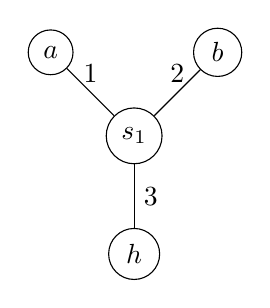
\begin{tikzpicture}[node distance={15mm},main/.style = {draw, circle}]
            \node[main] (s) {$s_1$};
            \node[main] (h) [below of=s] {$h$};
            \node[main] (a) [above left of=s]{$a$};
            \node[main] (b) [above right of=s]{$b$};
            \draw (a) --  node[above]{1}(s);
            \draw (b) --  node[above]{2}(s);
            \draw (s) --  node[right]{3}(h);
        \end{tikzpicture}
    \end{center}
    Correct Behavior:
    \begin{itemize}
        \item Forwarding from $a$ to $h$
        \item Forwarding from $b$ to $h$
        \item Limit traffic on link 3 (at most one packet)
    \end{itemize}
\end{frame}

\begin{frame}
    \begin{center}
        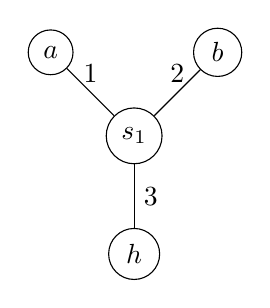
\begin{tikzpicture}[node distance={15mm},main/.style = {draw, circle}]
            \node[main] (s) {$s_1$};
            \node[main] (h) [below of=s] {$h$};
            \node[main] (a) [above left of=s]{$a$};
            \node[main] (b) [above right of=s]{$b$};
            \draw (a) --  node[above]{1}(s);
            \draw (b) --  node[above]{2}(s);
            \draw (s) --  node[right]{3}(h);
        \end{tikzpicture}
    \end{center}
    Events:
    \begin{itemize}
        \item $a$: forwarding packet from 1 to 3
        \item $b$: forwarding packet from 2 to 3
        \item $c$: detecting congestion on link 3
    \end{itemize}
    Event Structure:
    \begin{align*}
        \e \vdash a, \e \vdash b, \s{a,b} \vdash c
    \end{align*}
\end{frame}

\begin{frame}
    \begin{center}
        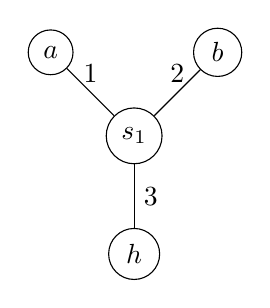
\begin{tikzpicture}[node distance={15mm},main/.style = {draw, circle}]
            \node[main] (s) {$s_1$};
            \node[main] (h) [below of=s] {$h$};
            \node[main] (a) [above left of=s]{$a$};
            \node[main] (b) [above right of=s]{$b$};
            \draw (a) --  node[above]{1}(s);
            \draw (b) --  node[above]{2}(s);
            \draw (s) --  node[right]{3}(h);
        \end{tikzpicture}
        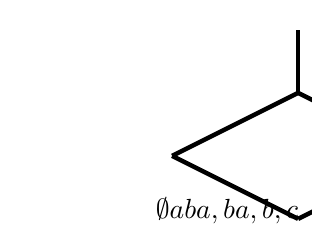
\begin{tikzpicture}[scale=0.8]
            \crd{0}{0}{$\emptyset$}
            \crd[above]{-2}{1}{$\s{a}$}
            \crd[above]{2}{1}{$\s{b}$}
            \crd[left]{0}{2}{$\s{a,b}$}
            \crd[left]{0}{3}{$\s{a,b,c}$}
            \draw [ultra thick] (0,0) -- (-2,1);
            \draw [ultra thick] (0,0) -- (2,1);
            \draw [ultra thick] (-2,1) -- (0,2);
            \draw [ultra thick] (2,1) -- (0,2);
            \draw [ultra thick] (0,2) -- (0,3);
        \end{tikzpicture}
    \end{center}
    \begin{itemize}
        \item Counterexample: $\sigma = \s{a,b,c}$
        \item Cause: $C(a,b) = \F$
        \item Conditions:
              \begin{align*}
                  \m & \vDash C(a,b) = \F \wedge \sigma \in
                  \mathcal{F}(\mathrm{E})                    \\
                  \m & \vDash [C(a,b)\la \T] \sigma \not \in
                  \mathcal{F}(\mathfrak{E}(\vec V)) \wedge \vec V = \vec v
                  \wedge \vec v \in \mathcal{E}
              \end{align*}
    \end{itemize}
\end{frame}

\begin{frame}
    \begin{center}
        \begin{tikzpicture}[node distance=20mm]
            \node[b] (eabc) {$EN(\s{a,b},c)$};
            \node[r] (ebc) [above left of=eabc] {$EN(\s{b},c)$};
            \node[r] (eac) [left of=ebc] {$EN(\s{a},c)$};
            \node[r] (eec) [above right of=eac,left of=ebc] {$EN(\e,c)$};
            \node[r] (mac) [above left of=eec] {$M(\s{a},c)$};
            \node[r] (mbc) [above right of=eec] {$M(\s{b},c)$};
            \node[r] (mec) [above left of=mbc] {$M(\e,c)$};
            \node[b] (mabc) [above right of=eabc] {$M(\s{a,b},c)$};
            \node[r] (cab) [above left of=mabc] {$C(a,b)$};
            \draw [->] (mec) -- (mac);
            \draw [->] (mec) -- (eec);
            \draw [->] (mec) -- (mbc);
            \draw [->] (mac) -- (eac);
            \draw [->] (mbc) -- (ebc);
            \draw [->] (mbc) -| (mabc);
            \draw [->] (eec) -- (eac);
            \draw [->] (eec) -- (ebc);
            \draw [->] (eac) -- (eabc);
            \draw [->] (ebc) -- (eabc);
            \draw [->] (cab) -- (eabc);
            \draw [->] (cab) -- (mabc);
            \draw [->] (mabc) edge (eabc);
            \draw [->] (mec) -- (2,5.6) -- (mabc);
            \draw [->] (mac) -- (-3,6) -- (3,6) -- (3,2.5) -- (mabc);
        \end{tikzpicture}
    \end{center}
\end{frame}

\begin{frame}
    \begin{center}
        \begin{tikzpicture}[node distance=20mm]
            \node[b] (eabc) {$EN(\s{a,b},c)$};
            \node[r] (ebc) [above left of=eabc] {$EN(\s{b},c)$};
            \node[r] (eac) [left of=ebc] {$EN(\s{a},c)$};
            \node[r] (eec) [above right of=eac,left of=ebc] {$EN(\e,c)$};
            \node[r] (mac) [above left of=eec] {$M(\s{a},c)$};
            \node[r] (mbc) [above right of=eec] {$M(\s{b},c)$};
            \node[r] (mec) [above left of=mbc] {$M(\e,c)$};
            \node[b] (mabc) [above right of=eabc] {$M(\s{a,b},c)$};
            \node[o] (cab) [above left of=mabc] {$C(a,b)$};
            \draw [->] (mec) -- (mac);
            \draw [->] (mec) -- (eec);
            \draw [->] (mec) -- (mbc);
            \draw [->] (mac) -- (eac);
            \draw [->] (mbc) -- (ebc);
            \draw [->] (mbc) -| (mabc);
            \draw [->] (eec) -- (eac);
            \draw [->] (eec) -- (ebc);
            \draw [->] (eac) -- (eabc);
            \draw [->] (ebc) -- (eabc);
            \draw [->] (cab) -- (eabc);
            \draw [->] (cab) -- (mabc);
            \draw [->] (mabc) edge (eabc);
            \draw [->] (mec) -- (2,5.6) -- (mabc);
            \draw [->] (mac) -- (-3,6) -- (3,6) -- (3,2.5) -- (mabc);
        \end{tikzpicture}
    \end{center}
\end{frame}

\begin{frame}
    \begin{center}
        \begin{tikzpicture}[node distance=20mm]
            \node[o] (eabc) {$EN(\s{a,b},c)$};
            \node[r] (ebc) [above left of=eabc] {$EN(\s{b},c)$};
            \node[r] (eac) [left of=ebc] {$EN(\s{a},c)$};
            \node[r] (eec) [above right of=eac,left of=ebc] {$EN(\e,c)$};
            \node[r] (mac) [above left of=eec] {$M(\s{a},c)$};
            \node[r] (mbc) [above right of=eec] {$M(\s{b},c)$};
            \node[r] (mec) [above left of=mbc] {$M(\e,c)$};
            \node[o] (mabc) [above right of=eabc] {$M(\s{a,b},c)$};
            \node[b] (cab) [above left of=mabc] {$C(a,b)$};
            \draw [->] (mec) -- (mac);
            \draw [->] (mec) -- (eec);
            \draw [->] (mec) -- (mbc);
            \draw [->] (mac) -- (eac);
            \draw [->] (mbc) -- (ebc);
            \draw [->] (mbc) -| (mabc);
            \draw [->] (eec) -- (eac);
            \draw [->] (eec) -- (ebc);
            \draw [->] (eac) -- (eabc);
            \draw [->] (ebc) -- (eabc);
            \draw [->] (cab) -- (eabc);
            \draw [->] (cab) -- (mabc);
            \draw [->] (mabc) edge (eabc);
            \draw [->] (mec) -- (2,5.6) -- (mabc);
            \draw [->] (mac) -- (-3,6) -- (3,6) -- (3,2.5) -- (mabc);
        \end{tikzpicture}
    \end{center}
\end{frame}

\begin{frame}
    \begin{center}
        \begin{tikzpicture}[node distance=20mm]
            \node[r] (eabc) {$EN(\s{a,b},c)$};
            \node[r] (ebc) [above left of=eabc] {$EN(\s{b},c)$};
            \node[r] (eac) [left of=ebc] {$EN(\s{a},c)$};
            \node[r] (eec) [above right of=eac,left of=ebc] {$EN(\e,c)$};
            \node[r] (mac) [above left of=eec] {$M(\s{a},c)$};
            \node[r] (mbc) [above right of=eec] {$M(\s{b},c)$};
            \node[r] (mec) [above left of=mbc] {$M(\e,c)$};
            \node[r] (mabc) [above right of=eabc] {$M(\s{a,b},c)$};
            \node[b] (cab) [above left of=mabc] {$C(a,b)$};
            \draw [->] (mec) -- (mac);
            \draw [->] (mec) -- (eec);
            \draw [->] (mec) -- (mbc);
            \draw [->] (mac) -- (eac);
            \draw [->] (mbc) -- (ebc);
            \draw [->] (mbc) -| (mabc);
            \draw [->] (eec) -- (eac);
            \draw [->] (eec) -- (ebc);
            \draw [->] (eac) -- (eabc);
            \draw [->] (ebc) -- (eabc);
            \draw [->] (cab) -- (eabc);
            \draw [->] (cab) -- (mabc);
            \draw [->] (mabc) edge (eabc);
            \draw [->] (mec) -- (2,5.6) -- (mabc);
            \draw [->] (mac) -- (-3,6) -- (3,6) -- (3,2.5) -- (mabc);
        \end{tikzpicture}
    \end{center}
\end{frame}

\begin{frame}
    \begin{align*}
        \m & \vDash EN(\e,a)       = \T              &
        \m & \vDash[C(a,b)\la T] EN(\e,a)       = \T   \\
        \m & \vDash EN(\s{b},a)    = \T              &
        \m & \vDash[C(a,b)\la T] EN(\s{b},a)    = \T   \\
        \m & \vDash EN(\s{c},a)    = \T              &
        \m & \vDash[C(a,b)\la T] EN(\s{c},a)    = \T   \\
        \m & \vDash EN(\s{b,c},a)  = \T              &
        \m & \vDash[C(a,b)\la T] EN(\s{b,c},a)  = \T   \\
        \m & \vDash EN(\e,b)       = \T              &
        \m & \vDash[C(a,b)\la T] EN(\e,b)       = \T   \\
        \m & \vDash EN(\s{a},b)    = \T              &
        \m & \vDash[C(a,b)\la T] EN(\s{a},b)    = \T   \\
        \m & \vDash EN(\s{c},b)    = \T              &
        \m & \vDash[C(a,b)\la T] EN(\s{c},b)    = \T   \\
        \m & \vDash EN(\s{a,c},b)  = \T              &
        \m & \vDash[C(a,b)\la T] EN(\s{a,c},b)  = \T   \\
        \m & \vDash EN(\e,c)       = \F              &
        \m & \vDash[C(a,b)\la T] EN(\e,c)       = \F   \\
        \m & \vDash EN(\s{a},c)    = \F              &
        \m & \vDash[C(a,b)\la T] EN(\s{a},c)    = \F   \\
        \m & \vDash EN(\s{b},c)    = \F              &
        \m & \vDash[C(a,b)\la T] EN(\s{b},c)    = \F   \\
        \m & \vDash EN(\s{a,b},c)  = \T              &
        \m & \vDash[C(a,b)\la T] EN(\s{a,b},c)
        = \textcolor{orange}{\F}                      \\
    \end{align*}
\end{frame}

\begin{frame}
    \begin{center}
        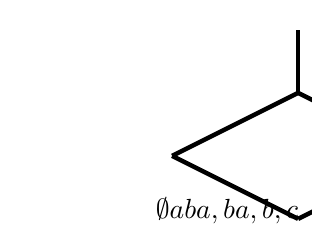
\begin{tikzpicture}[scale=0.8]
            \crd{0}{0}{$\emptyset$}
            \crd[above]{-2}{1}{$\s{a}$}
            \crd[above]{2}{1}{$\s{b}$}
            \crd[left]{0}{2}{$\s{a,b}$}
            \crd[left]{0}{3}{$\s{a,b,c}$}
            \draw [ultra thick] (0,0) -- (-2,1);
            \draw [ultra thick] (0,0) -- (2,1);
            \draw [ultra thick] (-2,1) -- (0,2);
            \draw [ultra thick] (2,1) -- (0,2);
            \draw [ultra thick] (0,2) -- (0,3);
        \end{tikzpicture}
        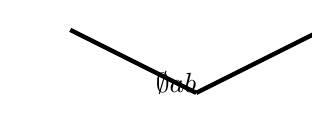
\begin{tikzpicture}[scale=0.8]
            \crd{0}{0}{$\emptyset$}
            \crd[above]{-2}{1}{$\s{a}$}
            \crd[above]{2}{1}{$\s{b}$}
            \draw [ultra thick] (0,0) -- (-2,1);
            \draw [ultra thick] (0,0) -- (2,1);
        \end{tikzpicture}
    \end{center}
\end{frame}